\section{Applications}
\subsection{Gamma Ray Concepts and Usages}
\begin{itemize}
    \item $\gamma$-rays (X-rays) are fingerprints of nuclei (atoms)
    \item The can be used in the following modes:
    \begin{itemize}
        \item Emission:\\
        Emission of gamma rays from the source provides information on the source itself, its environment, transport, and distribution.
        \item Induced emission:\\
        Provides information similar to above, but in examples such as NAA or XRF (see later sections).
        \item (Induced) Transmission or scattering:\\
        Transmission or scattering of photons provides information on the transmitting/ scattering object.
    \end{itemize}
\end{itemize}
\subsection{Carbon Dating}
\subsubsection{Assumptions and Concepts}
\begin{itemize}
    \item It is assumed that
    \begin{itemize}
        \item The rate of C-14 production is constant over time ($t\gg t_{1/2}$).
        \item The C-14 to C-12 ratio was in the same equilibrium as in the organisms today.
        \item The half-life of C-14 is known (measured to be 5730(40) years). Note: According to NNDC, the half-life is 5700(30) years.
    \end{itemize}
    \item C-14 is formed through $^{14}$N(n,p) from cosmic-ray produced neutrons.
    \item C-14 enters living organisms as CO$_2$, and can be found in all living organism with a constant C-14 to C-total ratio.
    \item The death of the organism sets the clock, and C-14 is depleted via beta decay.
\end{itemize}
\subsubsection{Measurement}
\begin{itemize}
    \item With the decay law,
    \begin{itemize}
        \item[] $N=N_0\exp(-\lambda t)$
        \item[] $\Rightarrow\;t=-\ln(N/N_0)/\lambda$
        \item[] $\Rightarrow\;t=\ln(C_0/C)\times t_{1/2}/\ln(2)$
        \item[] , where $C_0$ is the C-14 to C-total ratio when the organism died, and $C$ is the ratio measured in the sample. $C_0$ is assumed to be same as current living organisms. (This seems different from what is on the lecture slide, but I believe what is here is correct.)
    \end{itemize}
\end{itemize}
\subsubsection{Limitations}
\begin{itemize}
    \item The C-14 in samples have low specific activity:
    \begin{itemize}
        \item Low count rates even in living organsism
        \item Limited time range of $<50,000$ years (accelerator-based atomic mass spectrometry provides higher specificity, enabling ranges up to 100,000 years)
    \end{itemize}
    \item C-14 concentration changes over time:
    \begin{itemize}
        \item Global and local changes in cosmic ray flow and climate, etc. (e.g., increased use of fossil fuel and atmospheric nuclear testing)
        \item Independent calibration required for C-14 concentration
    \end{itemize}
    \item Method only sensitive to carbon-based living organisms
    \item Other radiometric dating techniques include K-Ar dating and U-Pb dating (both with half-life on the scale of $10^{9}$ years).
\end{itemize}
\subsection{Neutron Activation Analysis and X-Ray Fluorescence}
\subsubsection{Neutron Activation Analysis}
\begin{itemize}
    \item Coupled with gamma spectrometry, commonly used due to ease and low cost for determination of trace impurities ($\sim10^{-12}$) 
    \item Minimum-invasive, independent of chemical form
    \item Sensitivity varies due to differences in: 
    \begin{itemize}
        \item Neutron cross sections
        \item Natural isotopic abundances
        \item Half-lives
        \item Gamma-ray branching
    \end{itemize}
    \item Main constituents of living tissue (H, O, Si, P, S, Pb, Bi) cannot be detected
\end{itemize}
\subsubsection{X-Ray Fluorescence}
\begin{itemize}
    \item X-rays, $\gamma$-rays, or charged particles are used to excite atoms for emission of K or L shell X-rays.
    \item High resolution Si detectors enable XRF down to boron.
    \item Advantages over NAA include: small, self-contained units and no reactor irradiation required
    \item Can reach comparable relative sensitives as in NAA
\end{itemize}
\subsection{Gamma-Ray Spectroscopy and Imaging}
\subsubsection{Gamma-Ray Tracking}
\begin{figure}[ht]
    \centering
    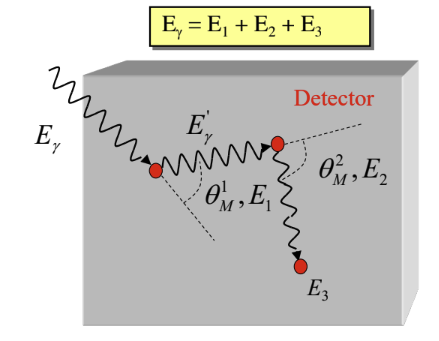
\includegraphics[width=0.4\textwidth]{images/gamma_ray_tracking.png}
    \caption{Concept of gamma-ray tracking.}
    \label{fig:gamma_ray_tracking}
\end{figure}
\begin{figure}[ht]
        \centering
        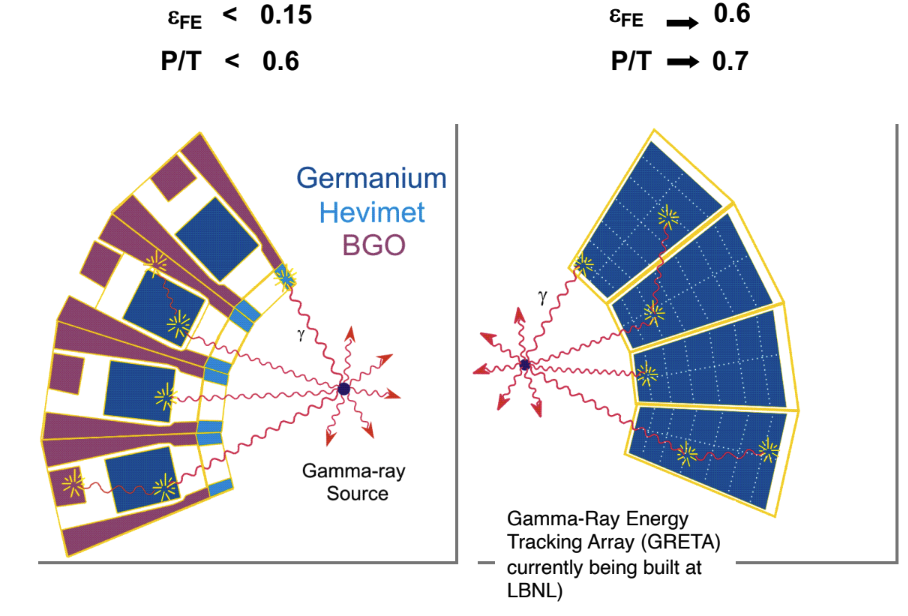
\includegraphics[width=0.6\textwidth]{images/gammasphere_GRETA.png}
        \caption{Configurations of Gammasphere (left) and GRETA (right).}
        \label{fig:gammasphere_GRETA}
    \end{figure}
\begin{itemize}
    \item Positions and energies of individual gamma-ray interactions are measured.
    \item The scattering sequence of interactions is measured.\\
    Assuming that the full energy $E_\gamma$ is deposited in the detector, for all possible $N!$ permutations of $N$ interactions, calculate the Compton scattering angle $\theta_C$ and compare with the measured values $\theta_M$ with a Figure-of-Merit ($\chi^2$). Select the sequence with minimum $\chi^2$. The process is summarized in figure~\ref{fig:gamma_ray_tracking}.
    \item While conventional gamma-ray detection provides only $E_\gamma$ with high $\epsilon_{FE}$ (efficiency), $P/T$ (peak-to-total ratio), and good $\Delta E$ (energy resolution), gamma-ray tracking detectors provide 3D positions with millimeter-scale resolution and energies of interactions in a correct time order. Improvements in the following aspects are also achieved:
    \begin{itemize}
        \item Rejects events with partial energy $\Rightarrow$ $P/T$
        \item Proper summing of multiple gamma-rays $\Rightarrow$ $P/T$ and $\epsilon_{FE}$
        \item Position of the first interaction $\Rightarrow$ Doppler correction
        \item Position of the first 2 interactions $\Rightarrow$ Compton imaging and polarization
        \item Reconstruction of full gamma-ray energy $\Rightarrow$ $P/T$ and $\epsilon_{FE}$
    \end{itemize}
    \item The upcoming gamma-ray tracking array is GRETA! See figure~\ref{fig:gammasphere_GRETA} for the comparison of GRETA and Gammasphere.
\end{itemize}
\subsubsection{Gamma-Ray Imaging}
\begin{itemize}
    \item Applied in astrophysics, medical imaging, and for security \& safety purposes.
    \item Collimators are used in attenuation to project gamma-ray emission onto the detector plane. Collimator-less cameras may use Compton imaging (with Compton-scattering kinematics and gamma-ray tracking to determine incident direction of gamma-ray) or angular correlation in photon emissions to determine the location of the emitting object (the $\sim180^\circ$ correlation of 511 keV annihilation photons). 
    \item SPECT and PET:
    \begin{enumerate}
        \item Single photon emission computed tomography (SPECT):
        \begin{itemize}
            \item The 3D distribution of radionuclides in an object is reconstructed using multiple 2D planar projections, as shown in figure~\ref{fig:SPECT}.
            \item The spatial resolution are typically 5$\sim$10 mm, with efficiency typcially 1$\sim$5$\times$10$^4$
        \end{itemize}
        \begin{figure}[ht]
            \centering
            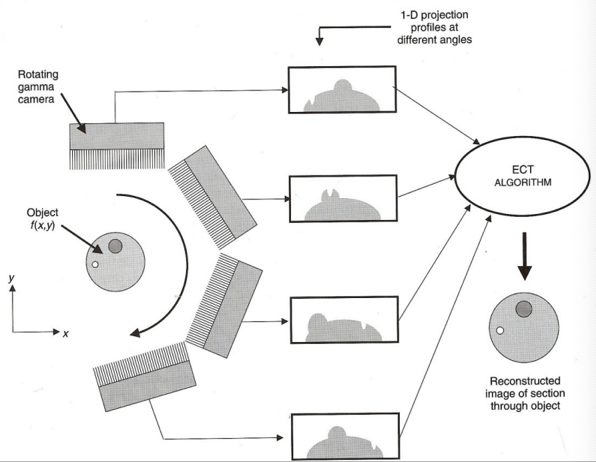
\includegraphics[width=0.5\textwidth]{images/SPECT.png}
            \caption{Concept of SPECT.}
            \label{fig:SPECT}
        \end{figure}
        \item Positron emission tomography (PET):
        \begin{itemize}
            \item Coincident measurement of the 2 characteristic annihilation 511 keV photons emitted in (nearly) opposite directions.
            \item The most important pharmaceutical is $^{18}$FDG.
            \item Combining PET (functional imaging) with X-ray Computed Tomography (CT) or Magnetic Resonance Imaging (MRI) (latter two are anatomical imaging) significantly enhances detection sensitivity.
            \item PET has the following properties when compared with SPECT:
            \begin{enumerate}
                \item No collimator required (``electronic'' collimation used only for scatter suppresion)
                \item 10 to 100 times higher sensitivity
                \item Resolution is limited by detector resolution (3$\sim$5 mm in clinical systems)
                \item Time coincidences and more complex electronics required
                \item Fast scintillators required to minimize coincident time
                \item More detectors required
                \item Since the photon energy is higher (511 keV), there is less attenuation, but thicker, more efficient detectors are required.
                \item The 511 keV photon detection is independent of the label ($^{11}$C, $^{18}$F, etc.)
            \end{enumerate}
        \end{itemize}
    \end{enumerate}
    \item Compton imaging
    \begin{itemize}
        \item Gamma-ray tracking used to determine the location of the source.
        \item To simplify position determination, the co-axial configurations are replaced with planar detectors: double-sided strip detectors (DSSD) built of HPGe, HPSi, Si(Li), CdTe, or CdZnTe. 
        \item No collimator is required; $\epsilon_{int}>1\%$.
        \item Designed to optimize angular resolution over efficiency: 1$\sim$2 degree angular resolution. 
    \end{itemize}
\end{itemize}